\documentclass{standalone}
\usepackage{tikz}
\usetikzlibrary{patterns, positioning}


\begin{document}
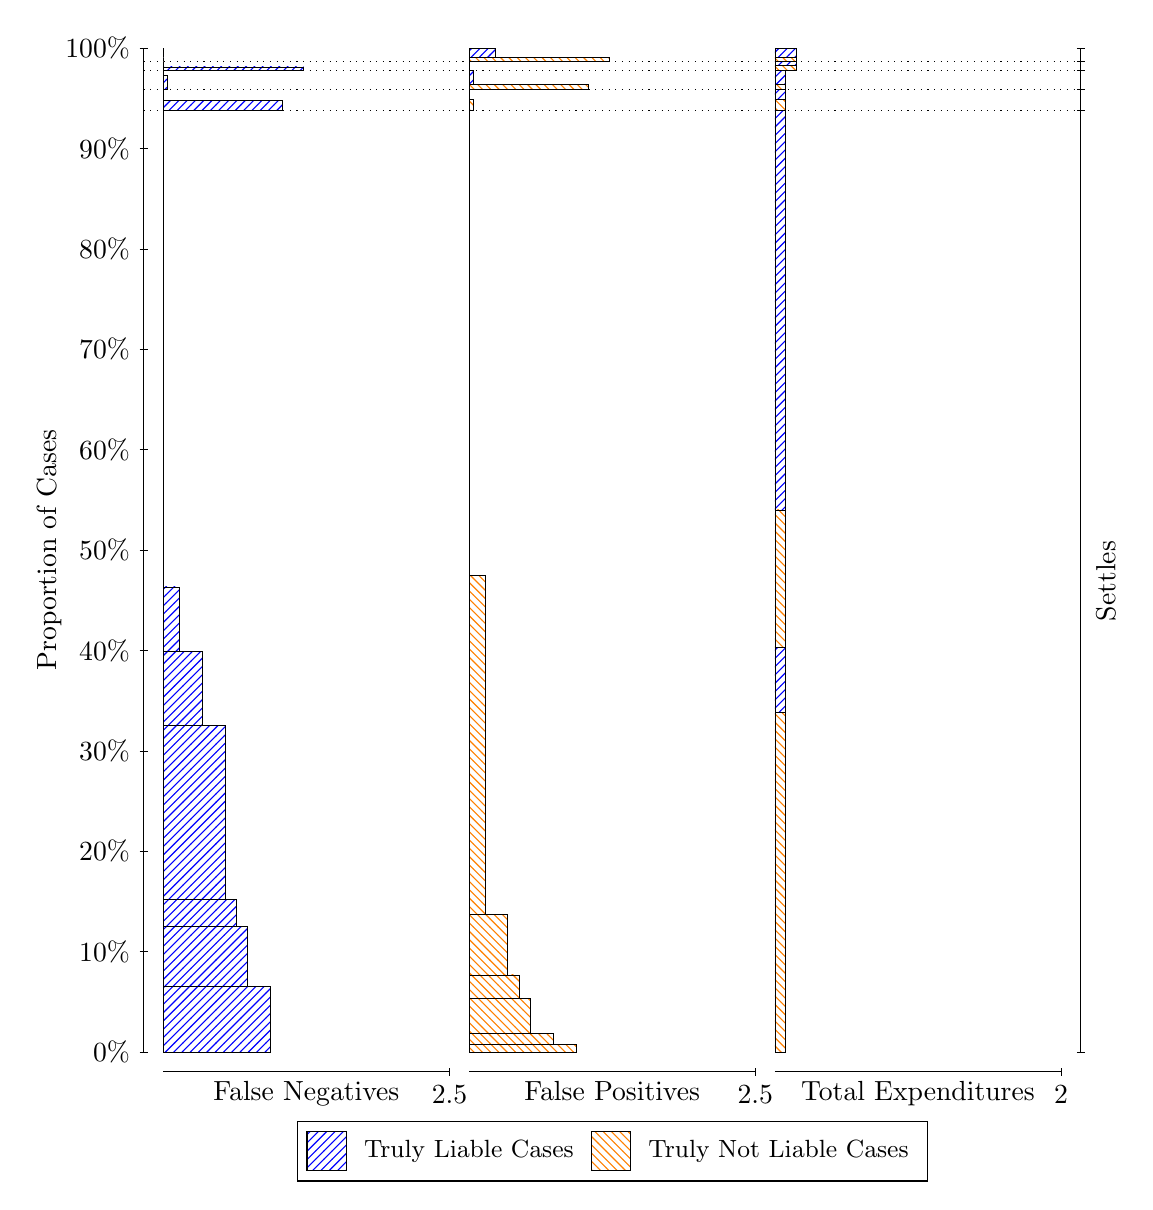
\begin{tikzpicture}
\draw[black, very thin] (1.5,1.75) -- (1.5,14.5);
\node[rotate=90, text=black, anchor=center] at (0.3, 8.125) {Proportion of Cases};
\draw[black, very thin] (1.45,1.75) -- (1.55,1.75);
\node[text=black, anchor=east] at (1.45, 1.75) {0\%};
\draw[black, very thin] (1.45,3.025) -- (1.55,3.025);
\node[text=black, anchor=east] at (1.45, 3.025) {10\%};
\draw[black, very thin] (1.45,4.3) -- (1.55,4.3);
\node[text=black, anchor=east] at (1.45, 4.3) {20\%};
\draw[black, very thin] (1.45,5.575) -- (1.55,5.575);
\node[text=black, anchor=east] at (1.45, 5.575) {30\%};
\draw[black, very thin] (1.45,6.85) -- (1.55,6.85);
\node[text=black, anchor=east] at (1.45, 6.85) {40\%};
\draw[black, very thin] (1.45,8.125) -- (1.55,8.125);
\node[text=black, anchor=east] at (1.45, 8.125) {50\%};
\draw[black, very thin] (1.45,9.4) -- (1.55,9.4);
\node[text=black, anchor=east] at (1.45, 9.4) {60\%};
\draw[black, very thin] (1.45,10.675) -- (1.55,10.675);
\node[text=black, anchor=east] at (1.45, 10.675) {70\%};
\draw[black, very thin] (1.45,11.95) -- (1.55,11.95);
\node[text=black, anchor=east] at (1.45, 11.95) {80\%};
\draw[black, very thin] (1.45,13.225) -- (1.55,13.225);
\node[text=black, anchor=east] at (1.45, 13.225) {90\%};
\draw[black, very thin] (1.45,14.5) -- (1.55,14.5);
\node[text=black, anchor=east] at (1.45, 14.5) {100\%};

\draw[black, very thin] (13.4,1.75) -- (13.4,14.5);
\draw[black, very thin] (13.35,1.75) -- (13.45,1.75);
\node[anchor=west] at (13.35, 1.75) {};
\draw[black, very thin] (13.35,13.711) -- (13.45,13.711);
\node[anchor=west] at (13.35, 13.711) {};
\draw[black, very thin] (13.35,13.974) -- (13.45,13.974);
\node[anchor=west] at (13.35, 13.974) {};
\draw[black, very thin] (13.35,14.212) -- (13.45,14.212);
\node[anchor=west] at (13.35, 14.212) {};
\draw[black, very thin] (13.35,14.332) -- (13.45,14.332);
\node[anchor=west] at (13.35, 14.332) {};
\draw[black, very thin] (13.35,14.5) -- (13.45,14.5);
\node[anchor=west] at (13.35, 14.5) {};

\draw[black, very thin, pattern color=blue, pattern=north east lines] (1.75,1.75) rectangle (3.1125,2.5788);
\draw[black, very thin, pattern color=blue, pattern=north east lines] (1.75,2.5788) rectangle (2.8218,3.3457);
\draw[black, very thin, pattern color=blue, pattern=north east lines] (1.75,3.3457) rectangle (2.6765,3.6836);
\draw[black, very thin, pattern color=blue, pattern=north east lines] (1.75,3.6836) rectangle (2.5312,5.9024);
\draw[black, very thin, pattern color=blue, pattern=north east lines] (1.75,5.9024) rectangle (2.2405,6.8399);
\draw[black, very thin, pattern color=blue, pattern=north east lines] (1.75,6.8399) rectangle (1.9498,7.6559);
\draw[black, very thin, pattern color=orange, pattern=north west lines] (1.75,7.6559) rectangle (1.75,13.711);
\draw[black, very thin, pattern color=blue, pattern=north east lines] (1.75,13.711) rectangle (3.2578,13.836);
\draw[black, very thin, pattern color=orange, pattern=north west lines] (1.75,13.836) rectangle (1.75,13.974);
\draw[black, very thin, pattern color=blue, pattern=north east lines] (1.75,13.974) rectangle (1.8045,14.15);
\draw[black, very thin, pattern color=orange, pattern=north west lines] (1.75,14.15) rectangle (1.75,14.212);
\draw[black, very thin, pattern color=blue, pattern=north east lines] (1.75,14.212) rectangle (3.5303,14.26);
\draw[black, very thin, pattern color=orange, pattern=north west lines] (1.75,14.26) rectangle (1.75,14.332);
\draw[black, very thin, pattern color=orange, pattern=north west lines] (1.75,14.332) rectangle (1.75,14.38);
\draw[black, very thin, pattern color=blue, pattern=north east lines] (1.75,14.38) rectangle (1.75,14.5);
\draw[black, very thin, pattern color=orange, pattern=north west lines] (5.6333,1.75) rectangle (6.9958,1.8472);
\draw[black, very thin, pattern color=orange, pattern=north west lines] (5.6333,1.8472) rectangle (6.7052,1.987);
\draw[black, very thin, pattern color=orange, pattern=north west lines] (5.6333,1.987) rectangle (6.4145,2.4261);
\draw[black, very thin, pattern color=orange, pattern=north west lines] (5.6333,2.4261) rectangle (6.2692,2.7288);
\draw[black, very thin, pattern color=orange, pattern=north west lines] (5.6333,2.7288) rectangle (6.1238,3.4958);
\draw[black, very thin, pattern color=orange, pattern=north west lines] (5.6333,3.4958) rectangle (5.8332,7.8052);
\draw[black, very thin, pattern color=blue, pattern=north east lines] (5.6333,7.8052) rectangle (5.6333,13.711);
\draw[black, very thin, pattern color=orange, pattern=north west lines] (5.6333,13.711) rectangle (5.6878,13.849);
\draw[black, very thin, pattern color=blue, pattern=north east lines] (5.6333,13.849) rectangle (5.6333,13.974);
\draw[black, very thin, pattern color=orange, pattern=north west lines] (5.6333,13.974) rectangle (7.1412,14.036);
\draw[black, very thin, pattern color=blue, pattern=north east lines] (5.6333,14.036) rectangle (5.6878,14.212);
\draw[black, very thin, pattern color=orange, pattern=north west lines] (5.6333,14.212) rectangle (5.6333,14.284);
\draw[black, very thin, pattern color=blue, pattern=north east lines] (5.6333,14.284) rectangle (5.6333,14.332);
\draw[black, very thin, pattern color=orange, pattern=north west lines] (5.6333,14.332) rectangle (7.4137,14.38);
\draw[black, very thin, pattern color=blue, pattern=north east lines] (5.6333,14.38) rectangle (5.9603,14.5);
\draw[black, very thin, pattern color=orange, pattern=north west lines] (9.5167,1.75) rectangle (9.6529,6.0595);
\draw[black, very thin, pattern color=blue, pattern=north east lines] (9.5167,6.0595) rectangle (9.6529,6.8883);
\draw[black, very thin, pattern color=orange, pattern=north west lines] (9.5167,6.8883) rectangle (9.6529,8.634);
\draw[black, very thin, pattern color=blue, pattern=north east lines] (9.5167,8.634) rectangle (9.6529,13.711);
\draw[black, very thin, pattern color=orange, pattern=north west lines] (9.5167,13.711) rectangle (9.6529,13.849);
\draw[black, very thin, pattern color=blue, pattern=north east lines] (9.5167,13.849) rectangle (9.6529,13.974);
\draw[black, very thin, pattern color=orange, pattern=north west lines] (9.5167,13.974) rectangle (9.6529,14.036);
\draw[black, very thin, pattern color=blue, pattern=north east lines] (9.5167,14.036) rectangle (9.6529,14.212);
\draw[black, very thin, pattern color=orange, pattern=north west lines] (9.5167,14.212) rectangle (9.7892,14.284);
\draw[black, very thin, pattern color=blue, pattern=north east lines] (9.5167,14.284) rectangle (9.7892,14.332);
\draw[black, very thin, pattern color=orange, pattern=north west lines] (9.5167,14.332) rectangle (9.7892,14.38);
\draw[black, very thin, pattern color=blue, pattern=north east lines] (9.5167,14.38) rectangle (9.7892,14.5);
\draw[black, dotted] (1.5,13.711) -- (13.4,13.711);
\draw[black, dotted] (1.5,13.974) -- (13.4,13.974);
\draw[black, dotted] (1.5,14.212) -- (13.4,14.212);
\draw[black, dotted] (1.5,14.332) -- (13.4,14.332);
\draw[black, very thin] (1.75,1.5) -- (5.3833,1.5);
\node[text=black, anchor=north] at (3.5667, 1.5) {False Negatives};
\draw[black, very thin] (5.3833,1.45) -- (5.3833,1.55);
\node[text=black, anchor=north] at (5.3833, 1.45) {2.5};

\draw[black, very thin] (5.6333,1.5) -- (9.2667,1.5);
\node[text=black, anchor=north] at (7.45, 1.5) {False Positives};
\draw[black, very thin] (9.2667,1.45) -- (9.2667,1.55);
\node[text=black, anchor=north] at (9.2667, 1.45) {2.5};

\draw[black, very thin] (9.5167,1.5) -- (13.15,1.5);
\node[text=black, anchor=north] at (11.333, 1.5) {Total Expenditures};
\draw[black, very thin] (13.15,1.45) -- (13.15,1.55);
\node[text=black, anchor=north] at (13.15, 1.45) {2};

\node[text=black, centered, rotate=90] at (13.72, 7.7306) {Settles};





\draw (7.449999999999999,1.5) node[draw=none] (baseCoordinate) {};
\begin{scope}[align=center]
        \matrix[scale=0.5, draw=black, below=0.5cm of baseCoordinate, nodes={draw}, column sep=0.1cm]{
            \node[rectangle, draw, minimum width=0.5cm, minimum height=0.5cm, pattern color=blue, pattern=north east lines] {}; &
            \node[draw=none, font=\small, text=black] (B) {Truly Liable Cases}; &
            \node[rectangle, draw, minimum width=0.5cm, minimum height=0.5cm, pattern color=orange, pattern=north west lines] {}; &
            \node[draw=none, font=\small, text=black] (B) {Truly Not Liable Cases}; \\
            };
\end{scope}

\end{tikzpicture}
\end{document}